\documentclass{article}

%package imports
\usepackage[dutch]{babel}
\usepackage[backend=biber,style=apa,autocite=inline]{biblatex}
\usepackage{wrapfig}
\usepackage{graphicx}

%meta data
\date{\today}
\title{ITIL Samenvatting}
\author{Wannes De creane, Michiel Schoofs}
\graphicspath{{./imgs/}}


%bib reference
\addbibresource{Bibliografie.bib}

%Custom commando's
\newcommand{\boldit}[1]{\emph{\textbf{#1}}} 
\newcommand{\customref}[1]{\underline{\ref{#1}: \nameref{#1}}}

\begin{document}

	\maketitle
	\section{Inleiding}
	ITIL staat voor Information Technology Infrastructure Library, Dit is een methodiek om aan procesmatig werken te doen binnen in IT. Meerbepaald een praktische “no nonsense approach”, zoals beschreven volgens ITIL®: the basics van \cite{Cater-Steel2006}, voor identificatie, planning, levering en support van IT services voor bedrijven.\\
	
	\par
	\noindent
	ITIL is aldus een leidraad om aan IT Service Management ( ITSM ) te doen, maar wat is dit nu juist? Een service voorziet waarde voor klanten, services die direct door klanten kunnen gebruikt worden noemt men bijgevolg business services een voorbeeld hiervan is bijvoorbeeld “Payroll”, dit is een IT service die gebruikt wordt om informatie bij te houden, compensatie te berekenen en cheques te genereren.\\
	
	\par
	\noindent
	Vaak ziet men de verschillende services van IT en business als een volledig andere wereld. Men gaat dan ook vaak gaan micromanagen en verliest het grote plaatje uit het oog. ITIL suggereert echter een meer holistische en consequente benadering van het ITSM process.\\
	
	\par
	\noindent
	Om de samenhang tussen nieuwe IT services en het bedrijf zonder problemen te laten werken zijn er dus verschillende processen nodig.
	
	\section{Situering van ITIL binnen Business}
	
	\begin{wrapfigure}{L}{0.3\textwidth}
		\centering
		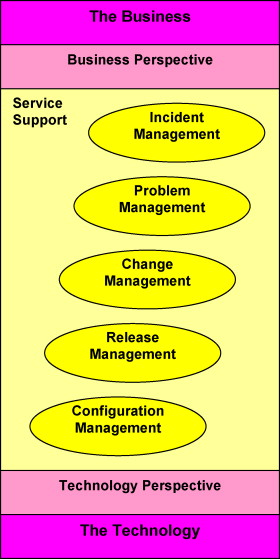
\includegraphics[width=0.25\textwidth]{itil1.jpg}
		\caption{\label{fig1:ItilProcess}This is a figure caption.}
	\end{wrapfigure}
	
	Zoals hierboven reeds kort uitgelegd is ITSM, een collectie van processen en normen voor het beheren,verbeteren en integreren van I.T. services binnen een bedrijf.\\ 
	
	\par
	\noindent
	Historisch gezien, zoals uitgelijnd in de paper van \cite{McNaughton_2010} waren meeste ITSM procedures gepatenteerd en bedrijfsspecifiek. Onder invloed van de ‘Office of Government Commerce’ kwam daar echter verandering in en werd ITIL ontwikkeld dit is een framework van ‘best practices’ om op een succesvolle en consequente manier aan ITSM te doen.\\
	
	\par
	\noindent
	Analoog met de devops beweging is het voornaamste doel om de kloof te dichten tussen I.T. en de bedrijfsvloer. Men ziet I.T. niet als een losstaande eenheid en probeert elke geleverde service op een succesvolle manier te integreren in het bedrijf. Ongeacht van het type (Hardware, software, support,...). De grafiek geeft dan ook een grafische weergave van het ITIL  process.\\
	
	\par
	\noindent
	Zoals aangegeven in Grafiek \ref{fig1:ItilProcess} ziet men opnieuw de twee grote categorieën naar voren komen namelijk de technologie en het bedrijf. Om het nog eens in andere woorden uit te drukken is ITIL de manier om het perspectief van het bedrijf en dat van nieuwe technologie in één lijn te brengen.\\
	
	\noindent
	Hieronder volgen dan ook enkele overzichten van de processen binnen ITIL.
	


	\printbibliography
\end{document}